% =====================================================================
%  System Integration section for the 2nd Year EOY Project Report.
%  Style matched to the reference report (article class, CM font, numbered
%  sections, bordered tables + captions). Compiles standalone; to merge into
%  the master report, drop the preamble and keep from \section onward (this is
%  intended as the section after "1 FDTD Solver and Physics").
%
%  Images live in docs/report/figures/ (see \graphicspath).
% =====================================================================
\documentclass[11pt]{article}
\usepackage[margin=1in]{geometry}
\usepackage{amsmath}
\usepackage{graphicx}
\graphicspath{{figures/}}   % block-diagram / screenshot images
\usepackage{xcolor}
\usepackage{array}
\usepackage{tikz}
\usetikzlibrary{positioning, arrows.meta}

\tikzset{
  blk/.style={draw, rounded corners, align=center, minimum height=7mm,
              inner xsep=4pt, inner ysep=3pt, font=\small},
  flow/.style={-{Stealth[length=2mm]}, thick},
  lbl/.style={font=\scriptsize\itshape, midway, align=center}
}

\title{System Integration, Control, and Demonstrations}
\author{}
\date{}

\begin{document}
\maketitle
\vspace{-3em}

% =====================================================================
\section{System Integration and Architecture}

The previous section described how a single FDTD cell is updated. This section
is about everything around that: how the solver, the wave source, the memory
buffers and the renderer are wired together into one working design on the
PYNQ--Z1, how the processor drives it all live, and what the finished system
actually shows on screen. The solver itself is treated here as a component with
a clean interface rather than re-explained.

% ---------------------------------------------------------------------
\subsection{System Overview}

At the top level the programmable logic is one long pipeline
(Fig.~\ref{fig:pipeline}). The source generator feeds the FDTD solver, the
solver's output is reduced to a per-cell field magnitude, that magnitude is
held in a double buffer, a bridge copies it into the renderer's memory, and the
renderer finally draws it out over HDMI. The guiding idea throughout is that
each stage is loosely coupled to its neighbours: because the solver and the
display naturally run at different and unrelated speeds, we never let one stage
read another's half-finished work. All field values are stored in signed Q3.13,
and the whole field datapath shares a single 25\,MHz clock so that there are no
clock-domain crossings on the path where data integrity matters most. Only the
3D renderer runs faster, at 100\,MHz, and we bring its pixels back into the
25\,MHz domain through an asynchronous FIFO.

\begin{figure}[h]
\centering
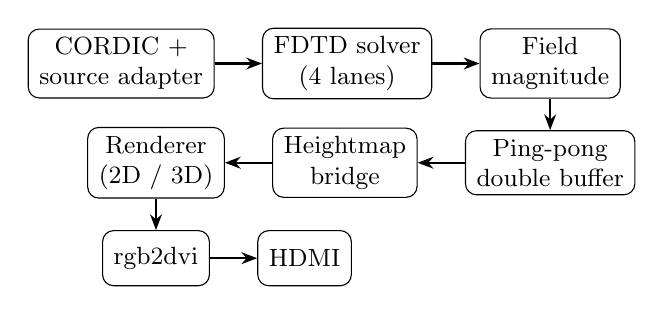
\begin{tikzpicture}[node distance=4mm and 6mm]
  \node[blk] (cor)  {CORDIC +\\source adapter};
  \node[blk, right=of cor] (fdtd) {FDTD solver\\(4 lanes)};
  \node[blk, right=of fdtd] (mag) {Field\\magnitude};
  \node[blk, below=of mag] (pp) {Ping-pong\\double buffer};
  \node[blk, left=of pp] (br) {Heightmap\\bridge};
  \node[blk, left=of br] (rend) {Renderer\\(2D / 3D)};
  \node[blk, below=of rend] (dvi) {rgb2dvi};
  \node[blk, right=of dvi] (hdmi) {HDMI};
  \draw[flow] (cor)--(fdtd); \draw[flow] (fdtd)--(mag); \draw[flow] (mag)--(pp);
  \draw[flow] (pp)--(br); \draw[flow] (br)--(rend); \draw[flow] (rend)--(dvi);
  \draw[flow] (dvi)--(hdmi);
\end{tikzpicture}
\caption{The end-to-end pipeline. Everything from the source generator to the
bridge shares one 25\,MHz clock; the renderer and HDMI serialiser follow on.}
\label{fig:pipeline}
\end{figure}

% ---------------------------------------------------------------------
\subsection{Building the Design from a Script}

Rather than wiring the design together by hand in Vivado's graphical
block-design editor, we generate the whole thing from a Tcl script. The reason
is the same one that leads any software project to version-control its source
rather than its binaries: the block-design file Vivado produces is a large,
auto-generated XML blob that cannot sensibly be reviewed or merged, whereas a
script is readable, diffable, and regenerates an identical bitstream every time.
We therefore commit the HDL and the script and treat them as the single source
of truth, which also makes it cheap to keep several design variants that differ
by only a few lines.

The script runs in the phases of Fig.~\ref{fig:build}. Our own modules are first
packaged as Vivado IP so they can be dropped onto the canvas; the renderer is
instead added as a \emph{module reference}, which has the quirk of requiring a
Verilog (not SystemVerilog) top-level wrapper. One lesson worth recording is
that we give every peripheral an explicit fixed address: we originally relied on
Vivado's automatic assignment, which orders peripherals alphabetically, and
discovered that simply adding new blocks silently shifted all the existing ones
and broke the addresses the notebook was written against.

\begin{figure}[h]
\centering
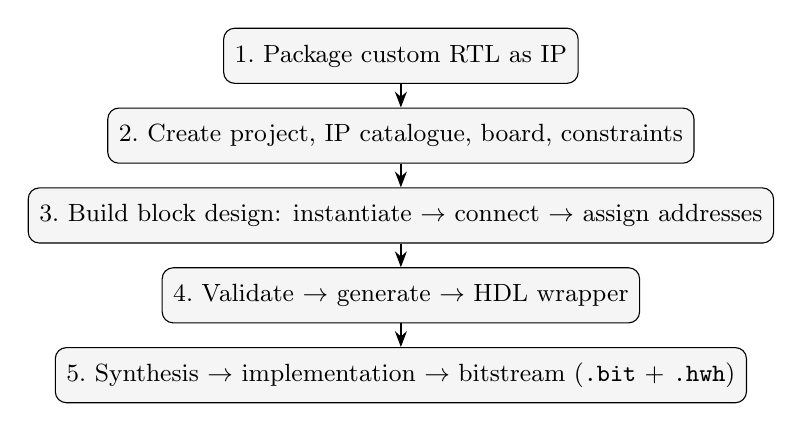
\begin{tikzpicture}[node distance=3mm]
  \node[blk, fill=black!4] (a) {1.\ Package custom RTL as IP};
  \node[blk, fill=black!4, below=of a] (b) {2.\ Create project, IP catalogue, board, constraints};
  \node[blk, fill=black!4, below=of b] (c) {3.\ Build block design: instantiate $\to$ connect $\to$ assign addresses};
  \node[blk, fill=black!4, below=of c] (d) {4.\ Validate $\to$ generate $\to$ HDL wrapper};
  \node[blk, fill=black!4, below=of d] (e) {5.\ Synthesis $\to$ implementation $\to$ bitstream (\texttt{.bit} + \texttt{.hwh})};
  \draw[flow] (a)--(b); \draw[flow] (b)--(c); \draw[flow] (c)--(d); \draw[flow] (d)--(e);
\end{tikzpicture}
\caption{The scripted build. Phases~1--4 always run; phase~5 is switched on by
an environment variable, so the same script builds either just the project or
the full bitstream.}
\label{fig:build}
\end{figure}

% ---------------------------------------------------------------------
\subsection{Clocking}

Every clock in the design comes from a single mixed-mode clock manager --- the
clocking wizard of Fig.~\ref{fig:clkwiz} --- fed by the board's 125\,MHz
reference (Table~\ref{tab:clocks}). Each domain has its own reset that is held
until the wizard asserts its \texttt{locked} output, so no block starts running
before its clock is stable. Where two domains have to meet we
handle the crossing deliberately rather than hoping for the best: an
asynchronous FIFO carries pixels from the 100\,MHz renderer into the 25\,MHz
scan-out, a dual-clock block RAM holds the heightmap written on one clock and
read on another, and the handful of control strobes that cross from the
processor's clock are passed through proper synchronisers.

\begin{table}[h]
\centering
\begin{tabular}{|l|l|}
\hline
Clock & Use \\
\hline
25\,MHz  & field datapath, 2D renderer, video timing \\
100\,MHz & 3D ray-march renderer core \\
125\,MHz & HDMI / TMDS serialiser \\
50\,MHz  & processor AXI register bus \\
\hline
\end{tabular}
\caption{Clock domains derived from the 125\,MHz board reference.}
\label{tab:clocks}
\end{table}

\begin{figure}[h]
\centering
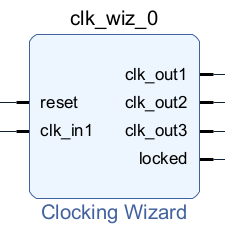
\includegraphics[width=0.32\linewidth]{clock_wizard.png}
\caption{The clocking wizard: one 125\,MHz input becomes the three on-chip
clocks, with a \texttt{locked} output that holds the resets until they are
stable.}
\label{fig:clkwiz}
\end{figure}

% ---------------------------------------------------------------------
\subsection{Generating the Source}

The wave is launched by a sinusoidal point source built from the two blocks in
Fig.~\ref{fig:cordic}. A Xilinx CORDIC core does the trigonometry --- it takes a
phase angle on its input stream and returns the sine and cosine --- and our
\texttt{cordic\_source\_adapter} wraps it into something the rest of the system
can use. The adapter accumulates the phase (advancing it one step per iteration,
which is what sets the source frequency), drives the AXI-Stream handshake to and
from the CORDIC, and scales the result by an amplitude the processor can change
on the fly. It can also inject the \emph{difference} of successive samples
rather than the raw sine: this carries no average value, which matters because a
moving source otherwise leaves a permanent ``trail'' of deposited energy behind
it.

\begin{figure}[h]
\centering
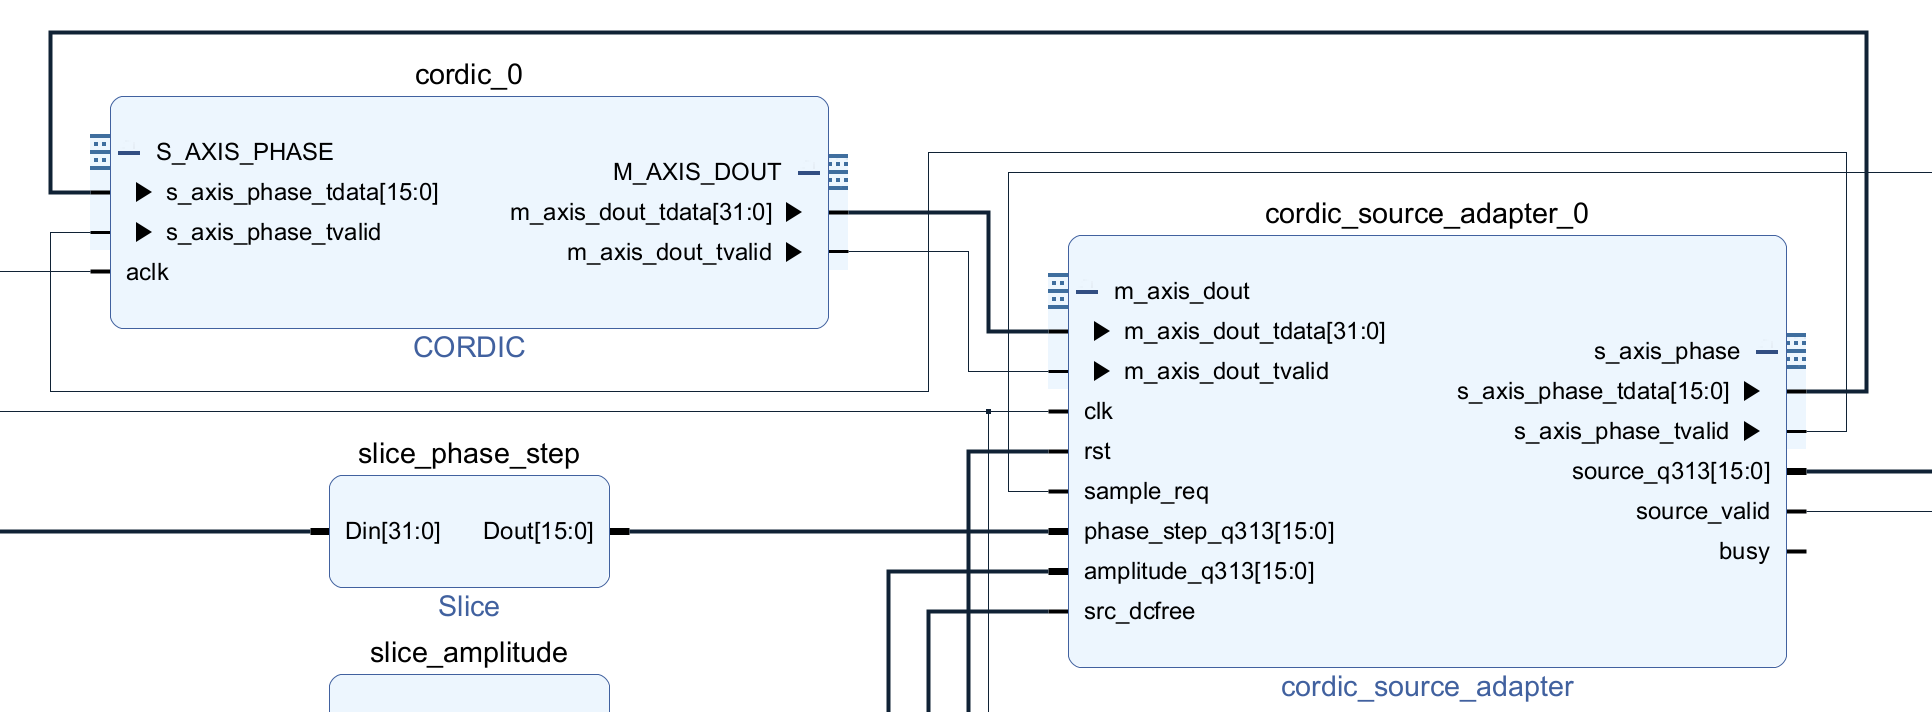
\includegraphics[width=\linewidth]{cordic_adaptor.png}
\caption{Block design of the source: the CORDIC core (left) feeds sine/cosine
over an AXI-Stream link into \texttt{cordic\_source\_adapter}, which the slice
blocks supply with the amplitude and phase-step set by the processor.}
\label{fig:cordic}
\end{figure}

% ---------------------------------------------------------------------
\subsection{The Moving Source and the Doppler Effect}

The system can also show a Doppler effect. If the source is made to travel
through the grid, the wavefronts compress ahead of it and stretch out behind, in
the same way a passing siren sounds higher in front and lower behind; past the
(numerical) wave speed the fronts can no longer move out of the way in time and
form a Mach cone. Producing this cleanly is as much an architectural decision as
a physical one, and it is a useful example of how work is divided between the
processor and the fabric.

The effect depends entirely on the source moving \emph{smoothly}: it advances
only a small fraction of a cell on each FDTD iteration --- we keep the position
to a resolution of $1/256$ of a cell --- and it has to do so in lockstep with
the solver, one small step for every iteration completed. This is precisely what
rules out driving the motion from the processor. The PS reaches the fabric only
over the AXI register bus through a Python loop, on a millisecond timescale,
whereas the solver finishes an iteration in microseconds; if the PS tried to
move the source itself it could manage only a few coarse jumps per second, too
slow and too granular, and the even wavefront spacing that produces the Doppler
effect would no longer be smooth.

The moving source therefore lives in the programmable logic. A small position
generator inside the FDTD adapter keeps the source coordinate in a fixed-point
accumulator, adds the velocity to it once per completed iteration, and reflects
it off the PML walls so the source bounces around inside the grid rather than
walking off the edge. The processor is left with the part it is actually suited
to: through the slice registers of Fig.~\ref{fig:slices} it sets the velocity,
arms the motion, and --- because the real hardware runs far faster than is
comfortable to watch --- throttles the iteration rate so the sweep is slow
enough to see. The PS decides \emph{what} the source should do; the PL is what
actually does it, iteration by iteration. That division of labour --- fast,
regular work in the fabric and slow, high-level choreography from the processor
--- is the same pattern that recurs throughout the design.

% ---------------------------------------------------------------------
\subsection{Decoupling the Solver and the Display}

This stage resolves a timing mismatch between the solver and the display. The
solver finishes a new frame whenever it happens to --- a rate that depends on the
grid size and how much we have slowed it for viewing --- while the renderer has
no such freedom: it must read a frame every twenty-fifth of a second to feed the
display. If we simply pointed the
renderer at the memory the solver was filling, it would now and then catch a
frame half-written, with the top of the screen showing the new frame and the
bottom the old one. This is the textbook producer--consumer problem, and we use
the textbook answer: two identical memories and a small controller
(Fig.~\ref{fig:pp}). At any moment one memory is being written by the solver and
the other is being read by the renderer; when the solver signals that a frame is
complete, the controller swaps the two roles in a single clock cycle, as
sketched in Fig.~\ref{fig:ppconcept}. Because the swap is atomic the renderer
always sees a whole, self-consistent frame, and because each memory is
dual-ported the reading and writing never collide. As both sides live in the
same 25\,MHz clock, none of this needs clock-crossing logic.

\begin{figure}[h]
\centering
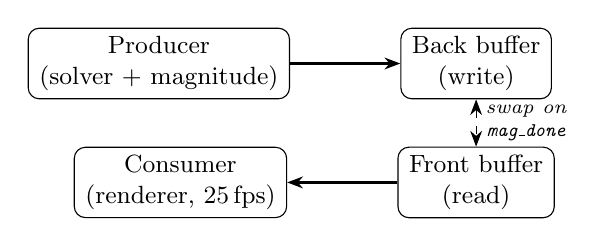
\begin{tikzpicture}[node distance=6mm and 14mm]
  \node[blk] (prod) {Producer\\(solver + magnitude)};
  \node[blk, right=of prod] (back) {Back buffer\\(write)};
  \node[blk, below=of back] (front) {Front buffer\\(read)};
  \node[blk, left=of front] (cons) {Consumer\\(renderer, 25\,fps)};
  \draw[flow] (prod)--(back); \draw[flow] (front)--(cons);
  \draw[{Stealth[length=2mm]}-{Stealth[length=2mm]}, dashed]
        (back) -- node[lbl, right]{swap on\\\texttt{mag\_done}} (front);
\end{tikzpicture}
\caption{The double-buffering idea: the producer fills the back buffer while the
consumer reads the front, and the two swap atomically each frame.}
\label{fig:ppconcept}
\end{figure}

\begin{figure}[h]
\centering
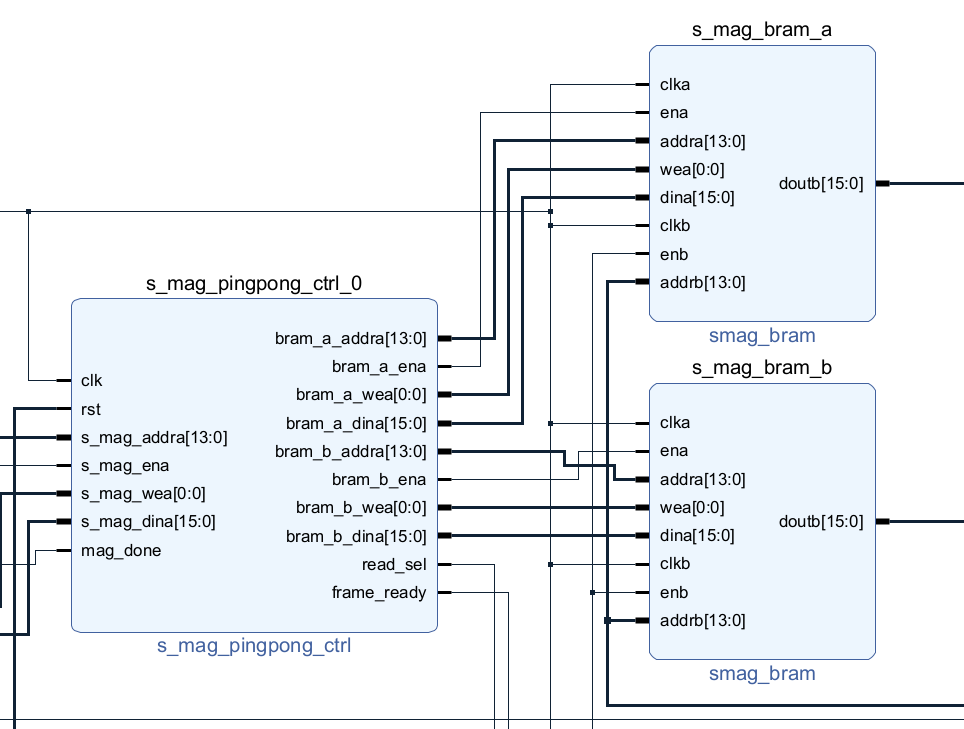
\includegraphics[width=0.8\linewidth]{ping-pong_buffer.png}
\caption{The same scheme in the block design: \texttt{s\_mag\_pingpong\_ctrl}
routes the solver's writes to whichever of the two \texttt{s\_mag} memories is
the current back buffer, and exports \texttt{read\_sel}/\texttt{frame\_ready} to
the reader.}
\label{fig:pp}
\end{figure}

% ---------------------------------------------------------------------
\subsection{The Bridge to the Renderer}

The renderer reads its terrain from its own private heightmap memories, so a
bridge (Fig.~\ref{fig:bridge}) copies each finished frame across. It does this
only during the display's vertical blanking interval, when the renderer is
issuing no reads, so the renderer can never catch the heightmap mid-update ---
the same tear-free principle as the double buffer, applied a second time. On the
way across it downsamples the $128\times128$ field to the $64\times64$ heightmap
and applies a height scale the processor can adjust live.

\begin{figure}[h]
\centering
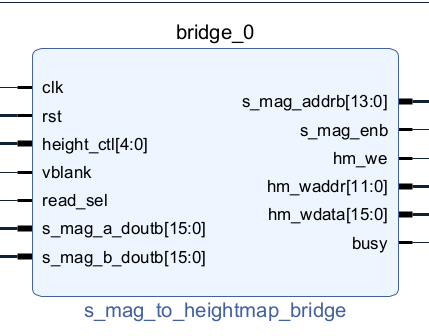
\includegraphics[width=0.5\linewidth]{s_mag_bridge.png}
\caption{The \texttt{s\_mag\_to\_heightmap\_bridge}: it reads the front buffer
(\texttt{read\_sel}, \texttt{s\_mag\_*\_doutb}), waits for \texttt{vblank}, and
writes the renderer heightmap (\texttt{hm\_we/waddr/wdata}).}
\label{fig:bridge}
\end{figure}

% ---------------------------------------------------------------------
\subsection{Driving It from the Processor}

Everything the operator touches goes through the processor's AXI bus
(Fig.~\ref{fig:psaxi}): the PS7 processing system drives an interconnect that
fans out to a set of simple GPIO register blocks, alongside a reset controller
that ties the whole AXI domain to the same locked clock. Because each GPIO
register is 32 bits wide but usually carries several smaller values, slice
blocks (Fig.~\ref{fig:slices}) split each register into the individual fields
the hardware consumes, and concatenation blocks gather status bits back into the
read-back word. The resulting map is given in Table~\ref{tab:axi}. Exposing the
controls this way is what makes the demonstration interactive: the operator
changes a value in the notebook and the simulation responds immediately, with no
rebuild.

\begin{figure}[h]
\centering
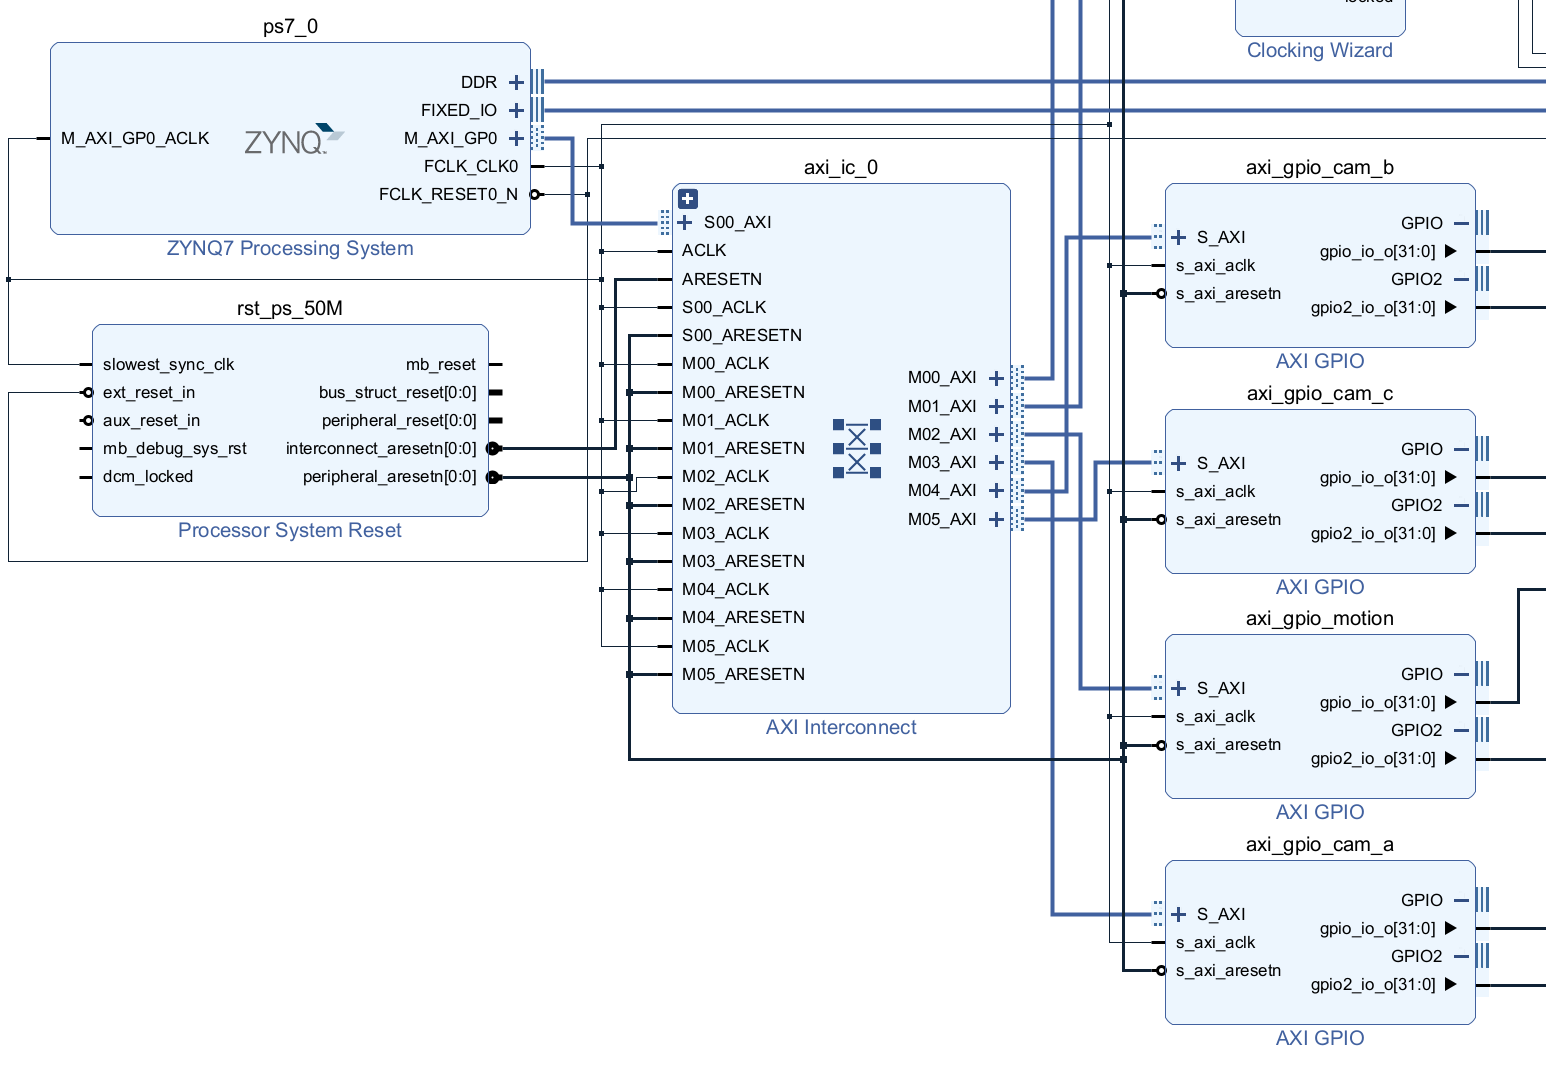
\includegraphics[width=\linewidth]{PS_axi_resets.png}
\caption{The processor (ZYNQ PS7) and its reset controller driving the AXI
interconnect, which fans out to the GPIO register blocks (control, motion,
status, and the camera channels).}
\label{fig:psaxi}
\end{figure}

\begin{figure}[h]
\centering
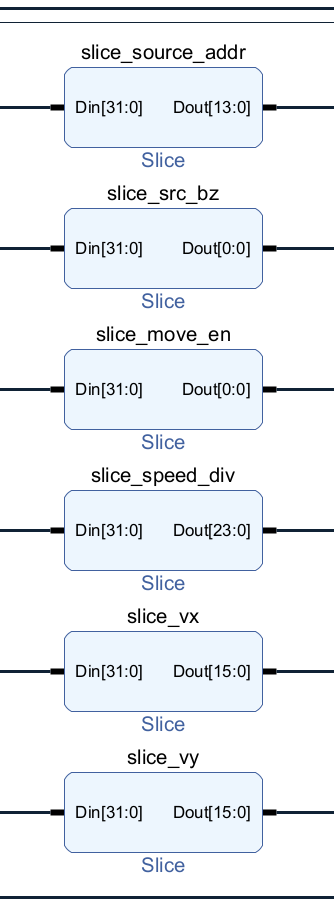
\includegraphics[width=0.28\linewidth]{slice_multisource.png}
\caption{Slice blocks unpacking a single 32-bit GPIO register into separate
control fields --- here the source address, source-field select, and the moving
-source velocity and throttle.}
\label{fig:slices}
\end{figure}

\begin{table}[h]
\centering
\begin{tabular}{|l|l|}
\hline
Address & Function \\
\hline
\texttt{0x41200000} & control: amplitude, frequency, source position, mode, clear \\
\texttt{0x41210000} & motion: source velocity, speed throttle, camera load \\
\texttt{0x41220000} & status (read-only): checksum and flags \\
\texttt{0x41230000}--\texttt{0x41250000} & camera basis (3D build) \\
\hline
\end{tabular}
\caption{The AXI-GPIO register map exposed to the notebook.}
\label{tab:axi}
\end{table}

% ---------------------------------------------------------------------
\subsection{Multi-Lane Parallelism}

To speed the solver up we split the grid into four horizontal \emph{lanes} and
update them in lockstep, each with its own copy of the field memories. One
iteration then takes 2048 cycles instead of 8192 --- four times faster, for an
identical result. The cost falls on memory rather than logic: each lane needs its
own memories and read ports, and neighbouring lanes exchange a single boundary
row, because the update at the edge of one lane reaches into the next. Notably the
four-lane version used \emph{fewer} block RAMs than the single-lane one (108
against 114), because four smaller memories pack into the device's RAM blocks more
tightly than one large one. We also evaluated eight and sixteen lanes but settled
on four: beyond that point the additional speed no longer justifies the growing
boundary-exchange logic and routing congestion, particularly as the solver was
already running well ahead of the display's frame rate.

% ---------------------------------------------------------------------
\subsection{The Two Demonstrations}

The same solver drives two different renderers, and the choice between them is
primarily a trade between block-RAM use and clock speed (Table~\ref{tab:demos}).
The first is a flat top-down contour heatmap (Fig.~\ref{fig:2d}). It needs only a
single heightmap memory, and freeing the rest of the block RAM is what allowed us
to quadruple the grid to $128\times128$ for finer detail; with the
source set moving it clearly shows the wavefronts bunching ahead and stretching
behind, the Doppler effect. The second renders the field as a shaded
three-dimensional landscape by ray-marching (Fig.~\ref{fig:3d}). This view is more
detailed but more resource-intensive --- it needs around fifty copies of the
heightmap --- so it runs at 100\,MHz and folds its memory reads across several
cycles to fit, and its camera can be orbited live from the notebook. Keeping both
is deliberate: the 2D view is the clearer one for reading the physics, and the 3D
view gives a more intuitive sense of the field's shape.

\begin{figure}[h]
\centering
\begin{minipage}[b]{0.46\linewidth}\centering
  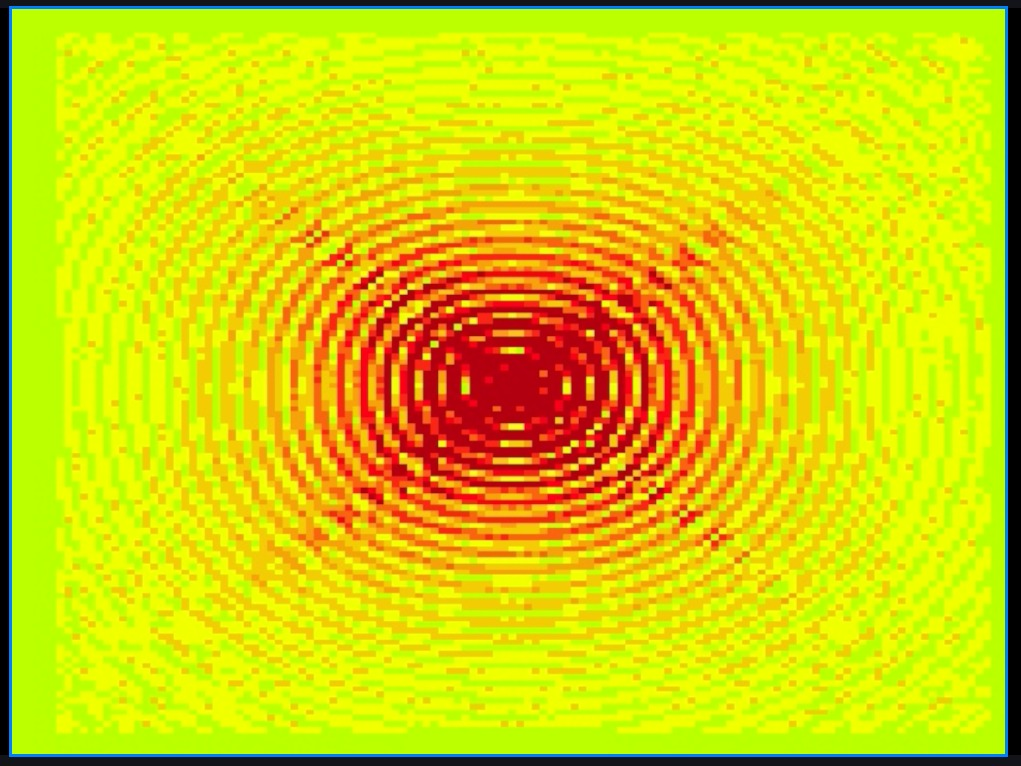
\includegraphics[width=\linewidth]{2D_image.png}
  \caption{2D contour heatmap: concentric wavefronts radiating from the point
  source.}
  \label{fig:2d}
\end{minipage}\hfill
\begin{minipage}[b]{0.50\linewidth}\centering
  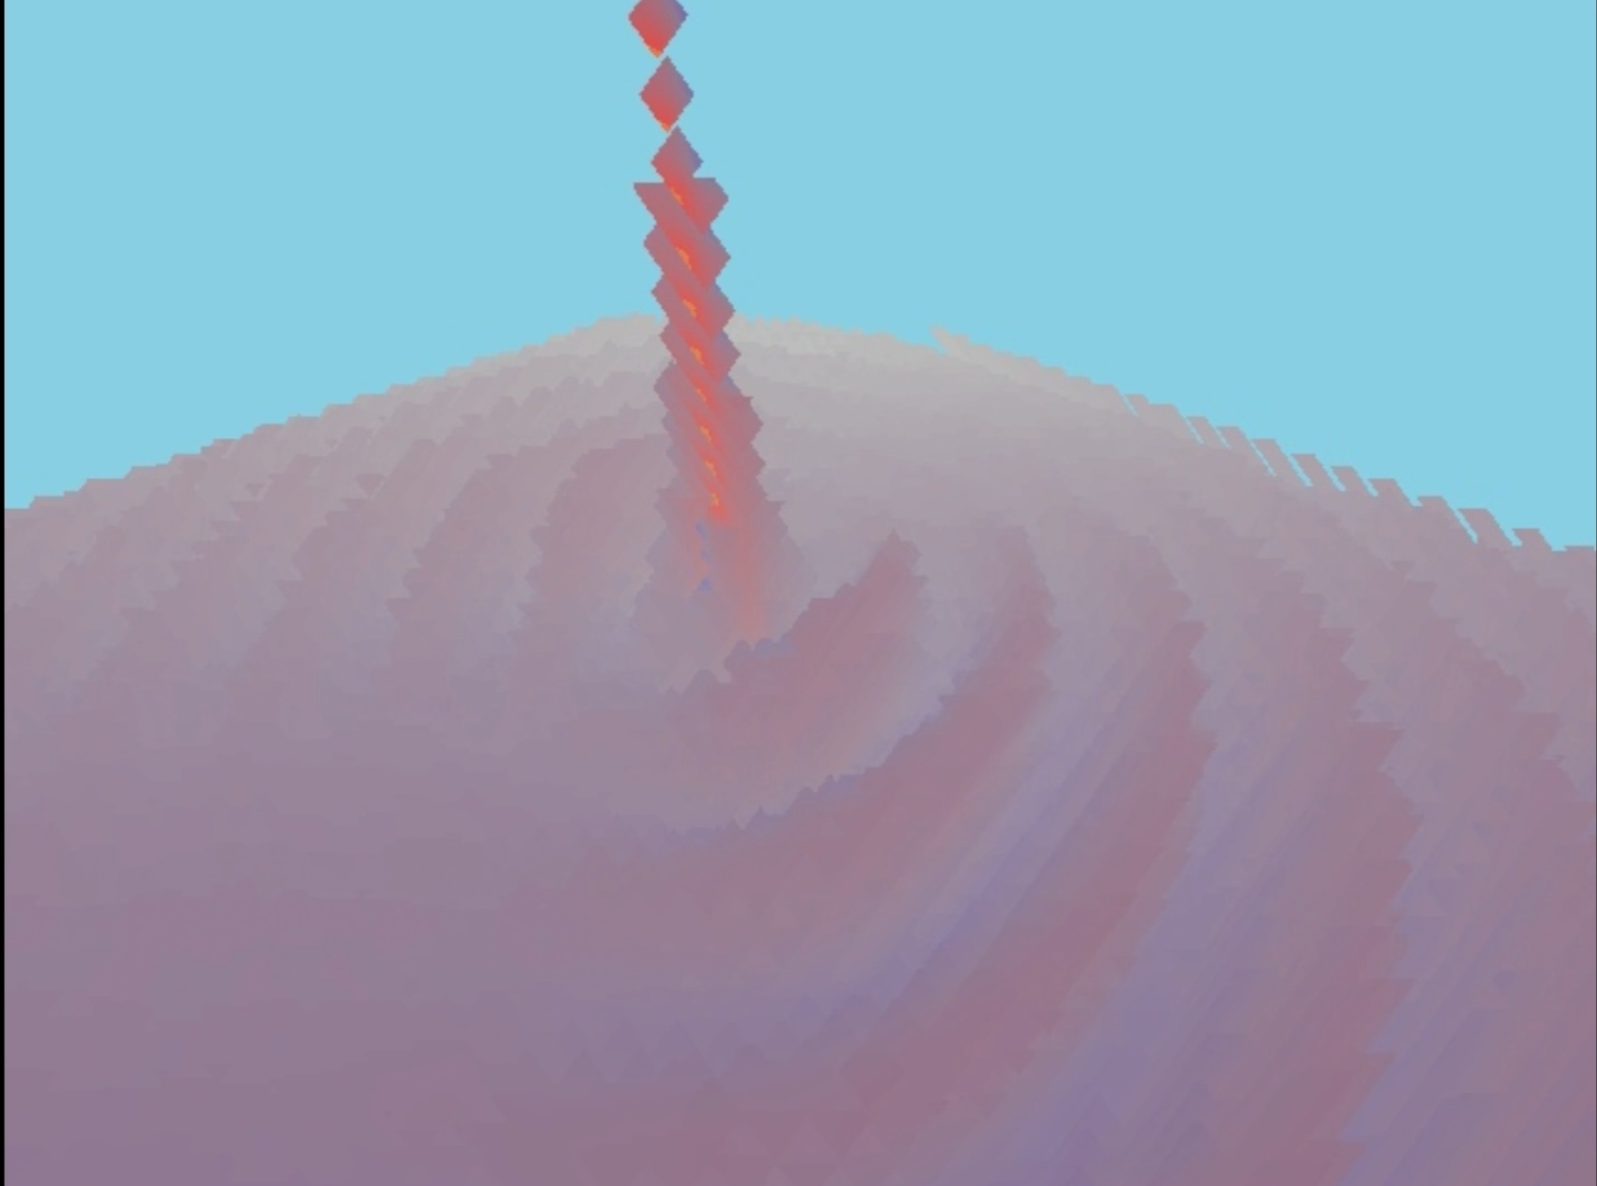
\includegraphics[width=\linewidth]{3D_image.png}
  \caption{3D ray-marched view: the field as a shaded heightmap, with the source
  rising at the centre.}
  \label{fig:3d}
\end{minipage}
\end{figure}

\begin{table}[h]
\centering
\begin{tabular}{|l|l|l|}
\hline
 & 2D contour & 3D ray-march \\
\hline
Heightmap BRAMs & 1            & $\sim$50 \\
Clock           & 25\,MHz      & 100\,MHz (1 px / 4 cyc) \\
Strength        & clarity, finer grid & visual impact, movable camera \\
Interaction     & moving source (Doppler) & orbiting camera \\
\hline
\end{tabular}
\caption{The two demonstrations and their block-RAM versus clock trade-off.}
\label{tab:demos}
\end{table}

\end{document}
